%$Id: chi06.tex,v 1.4 2006/02/13 23:19:21 rlw Exp rlw $
\documentclass[dvips]{beamer}
\usetheme[hideothersubsections]{Boston}
\usepackage{amsmath,amssymb,bm,array,graphicx,epic,hyperref,url,psfrag}
%\usepackage{movie15}
%\bibliographystyle{jasa}
\graphicspath{{./}{eps/}}
\setbeamercovered{transparent}
\title{Towards Objective Priors}
\subtitle{\Large in Nonparametric Regression and Classification}
\author[M. Clyde]{Merlise Clyde \\ (joint with Robert Wolpert and Zhi Ouyang)}
\institute{Department of Statistical Science \\ Duke
University }
\date{10th Annual Winter Workshop  \\ Bayesian Model Selection and
  Objective Methods \\Jan 11-12, 2008}
\newcommand{\bs}[2]{\begin{frame} \frametitle{#1} 
{#2}
\end{frame} }
\usepackage{amsmath,amssymb,array,eucal}
\usepackage{xcolor}
\definecolor{beamer@blendedblue}{RGB}{86,155,189}
\definecolor{myblue}{RGB}{12,76,138}
\setbeamercolor{structure}{fg=myblue}
\definecolor{Ftitle}{RGB}{12,76,138}
\definecolor{Descitem}{RGB}{238,238,244}
\definecolor{StdTitle}{RGB}{12,76,138}
\definecolor{StdBody}{RGB}{213,24,0}
\definecolor{StdBody}{RGB}{213,24,0}

\definecolor{AlTitle}{RGB}{255, 190, 190}
\definecolor{AlBody}{RGB}{213,24,0}

\definecolor{ExTitle}{RGB}{201, 217, 217}
\definecolor{ExBody}{RGB}{213,24,0}

\setbeamercolor{frametitle}{fg = Ftitle}
\setbeamercolor{title}{fg = Ftitle}
\setbeamercolor{item}{fg = Ftitle}
\setbeamercolor{subitem}{fg = Ftitle}
\setbeamercolor{subsubitem}{fg = Ftitle}
\setbeamercolor{description item}{fg = myblue}
\setbeamercolor{titlelike}{fg=myblue}
\newcommand{\e}{\mathbf{e}}
\renewcommand{\P}{\textsf{P}}
\newcommand{\R}{\textsf{R}}
\newcommand{\mat}[1] {\mathbf{#1}}
%\newcommand{\ind}{\mathrel{\mathop{\sim}\limits^{\mathit{ind}}}}
%\newcommand{\iid}{\mathrel{\mathop{\sim}\limits^{\mathit{iid}}}}
\newcommand{\E}{\textsf{E}}
\newcommand{\SE}{\textsf{SE}}
\newcommand{\SSE}{\textsf{SSE}}
\renewcommand{\SS}{\textsf{SS}}
\newcommand{\MSE}{\textsf{MSE}}
\newcommand{\SSR}{\textsf{SSR}}
\newcommand{\Be}{\textsf{Beta}}
\newcommand{\St}{\textsf{St}}
%\newcommand{\C}{\textsf{C}}
\newcommand{\GDP}{\textsf{GDP}}
\newcommand{\NcSt}{\textsf{NcSt}}
\newcommand{\Bin}{\textsf{Bin}}
\newcommand{\NB}{\textsf{NegBin}}
\renewcommand{\NG}{\textsf{NG}}
\newcommand{\N}{\textsf{N}}
\newcommand{\Ber}{\textsf{Ber}}
\newcommand{\Poi}{\text{Poi}}
\newcommand{\Gam}{\textsf{Gamma}}
\newcommand{\Gm}{\textsf{G}}
\newcommand{\Un}{\textsf{Unif}}
\newcommand{\Ex}{\textsf{Exp}}
\newcommand{\DE}{\textsf{DE}}
\newcommand{\tr}{\textsf{tr}}
\newcommand{\cF}{{\cal{F}}}
\newcommand{\cL}{{\cal{L}}}
\newcommand{\cI}{{\cal{I}}}
\newcommand{\cB}{{\cal{B}}}
\newcommand{\cP}{{\cal{P}}}
\newcommand{\bbR}{\mathbb{R}}
\newcommand{\bbN}{\mathbb{N}}
\newcommand{\pperp}{\mathrel{{\rlap{$\,\perp$}\perp\,\,}}}
\newcommand{\OFP}{(\Omega,\cF, \P)}
\newcommand{\eps}{\boldsymbol{\epsilon}}
\newcommand{\1}{\mathbf{1}_n}
\newcommand{\gap}{\vspace{8mm}}
\newcommand{\ind}{\mathrel{\mathop{\sim}\limits^{\rm ind}}}
\newcommand{\simiid}{\ensuremath{\mathrel{\mathop{\sim}\limits^{\rm
iid}}}}
\newcommand{\eqindis}{\ensuremath{\mathrel{\mathop{=}\limits^{\rm D}}}}
\newcommand{\iid}{\textit{i.i.d.}}
\newcommand{\SSZ}{S_{zz}}
\newcommand{\SZW}{S_{zw}}
\newcommand{\Bias}{\textsf{Bias}}
\newcommand{\Var}{\textsf{Var}}
\newcommand{\corr}{\textsf{corr}}
\newcommand{\diag}{\textsf{diag}}
\newcommand{\var}{\textsf{var}}
\newcommand{\Cov}{\textsf{Cov}}
\newcommand{\Sam}{{\cal S}}
\def\H{\mathbf{H}}
\newcommand{\I}{\mathbf{I}}
\newcommand{\Y}{\mathbf{Y}}
\newcommand{\tY}{\tilde{\mathbf{Y}}}
\newcommand{\Yhat}{\hat{\mathbf{Y}}}
\newcommand{\Yobs}{\mathbf{Y}_{{\cal S}}}
\newcommand{\barYobs}{\bar{Y}_{{\cal S}}}
\newcommand{\barYmiss}{\bar{Y}_{{\cal S}^c}}
\def\bv{\mathbf{b}}
\def\X{\mathbf{X}}
\def\tX{\tilde{\mathbf{X}}}
\def\x{\mathbf{x}}
\def\xbar{\bar{\x}}
\def\Xg{\mathbf{X}_{\boldsymbol{\gamma}}}
\def\Ybar{\bar{Y}}
\def\ybar{\bar{y}}
\def\y{\mathbf{y}}
\def\Yf{\mathbf{Y_f}}
\def\W{\mathbf{W}}
\def\w{\mathbf{w}}
\def\U{\mathbf{U}}
\def\V{\mathbf{V}}
\def\Q{\mathbf{Q}}
\def\Z{\mathbf{Z}}
\def\z{\mathbf{z}}
\def\v{\mathbf{v}}
\def\u{\mathbf{u}}

\def\zero{\mathbf{0}}
\def\one{\mathbf{1}}
\newcommand{\taub}{\boldsymbol{\tau}}
\newcommand{\betav}{\boldsymbol{\beta}}
\newcommand{\alphav}{\boldsymbol{\alpha}}
\newcommand{\A}{\mathbf{A}}
\def\a{\mathbf{a}}
\newcommand{\B}{\mathbf{B}}
\def\b{\boldsymbol{\beta}}
\def\bhat{\hat{\boldsymbol{\beta}}}
\def\tb{\tilde{\boldsymbol{\beta}}}
\def\bg{\boldsymbol{\beta_\gamma}}
\def\bgnot{\boldsymbol{\beta_{(-\gamma)}}}
\def\mub{\boldsymbol{\mu}}
\def\tmub{\tilde{\boldsymbol{\mu}}}
\def\muhat{\hat{\boldsymbol{\mu}}}
\def\t{\boldsymbol{\theta}}
\def\tk{\boldsymbol{\theta}_k}
\def\tj{\boldsymbol{\theta}_j}
\def\Mk{\boldsymbol{{\cal M}}_k}
\def\M{{{\cal M}}}
\def\Mj{{{\cal M}}_j}
\def\Mi{{{\cal M}}_i}
\def\Mg{{\cal M}_\gamma}
\def\Mnull{{\cal M}_{N}}
\def\gMPM{\boldsymbol{\gamma}_{\text{MPM}}}
\def\gHPM{\boldsymbol{\gamma}_{\text{HPM}}}
\def\Mfull{\boldsymbol{{\cal M}}_{F}}
\def\tg{\boldsymbol{\theta}_{\boldsymbol{\gamma}}}
\def\g{\boldsymbol{\gamma}}
\def\eg{\boldsymbol{\eta}_{\boldsymbol{\gamma}}}
\def\G{\mathbf{G}}
\def\cM{\cal M}
\def\D{\Delta}
\def \shat{{\hat{\sigma}}^2}
\def\uv{\mathbf{u}}
\def\l {\lambda}
\def\d{\delta}
\def\Sigmab{\boldsymbol{\Sigma}}
\def\Lambdab{\boldsymbol{\Lambda}}
\def\lambdab{\boldsymbol{\lambda}}
\def\Mg{{\cal M}_\gamma}
\def\S{{\cal{S}}}
\def\qg{p_{\boldsymbol{\gamma}}}
\def\pg{p_{\boldsymbol{\gamma}}}
\def\t{\boldsymbol{\theta}}
\def\T{\boldsymbol{\Theta}}

\input{colornames}
\newcommand{\blue}{\textcolor{Blue}}
\newcommand{\green}{\textcolor{PineGreen}}
\newcommand{\purple}{\textcolor{Purple}}
\newcommand{\red}{\textcolor{RedOrange}}
\definecolor{aper}{rgb}{0.7412,0,1}
\definecolor{daily}{rgb}{0.1412,0,1}
\newcommand{\ap}{\textcolor{aper}}
\newcommand{\dy}{\textcolor{daily}}
\logo{
\includegraphics[width=.6in,height=.6in]{duke}}


\begin{document}
\begin{frame}
  \titlepage
\end{frame}
%\section[Outline]{}

%\bs{Outline}{
%\tableofcontents 
%}

\section{Nonparametric Regression}
\bs{Problem Setting}{
Consider the nonparametric regression problem with
data $\{Y_i, \bfx_i\} \quad i = 1, \dots n $
$$ \E[Y \mid \bfx] = f(\bfx), \quad \bfx \in \cfX$$


Prior Distributions on $f$:

\begin{itemize}
\item  Gaussian Process Priors
\item  Dirichlet Process priors
\item  Expansions of $f$  (finite and infinite)
\end{itemize}

}

\subsection{Expansions}
\bs{Basis Expansions} {
Need to place a prior distribution  on unknown function $f \in \cfF$

Expansions $f(\bfx_i) = \sum_j  \psi_j(\bfx_i)\beta_j$
 
  \begin{itemize}
   \item  $\{\psi_j\}$: basis functions for some
     function space $\cfF$ %(\eg, $L^2(\cfX,dx$)) 
   \item  $\{\beta_j\}$  unknown coefficients
   \item Commonly used basis functions:
 \begin{itemize}
 \item Polynomials
 \item Fourier 
 \item Splines 
 \item Wavelets 
 \item Kernels 
 \end{itemize} 
   \end{itemize}

}

\subsection{Over-complete Dictionaries }

\bs{Over-complete Dictionaries (OCD)} {
In recent years OCD have received considerable attention
\begin{itemize}
\item  Collection $\{\psi_{j}(\bfx) \}$  ``more than a basis''
  \item Examples:
    \begin{itemize}
    \item ``Large $p$, small $n$''
    \item Unions of two (or more) bases
    \item Translation Invariant Wavelets
      % $\phi_{j,k}(x) = |a|^{-j/2}\psi\left( \frac{x - k
      %     b}{a^j}\right) \quad j, k, \in \bbZ $;
    \item Free-knot splines
    \item Gabor frames
   % $\psi_{j,k}(x) = e^{2 \pi  i j b x} g( x - k a) \quad  j, k \in \bbZ$  ; 
   \item Kernels:  $\psi_j(\bfx) = k(\bfx; \bfomega_j)$ with kernel
   specific scale \& location parameters 
   \end{itemize}
\item   Expand $f$ in terms of OCD  
   \[ f(\bfx_i) = \sum_{j \in \cfJ } \psi_j(\bfx_i)\beta_j,\qquad f \in
   \bbF=\overline{\{\psi_{j}\}}\]
  \end{itemize} 
}


\bs{Why Over-complete Dictionaries?} {
  \begin{itemize}
  \item[$+$] More flexible - local adaptivity
  \item[$+$] Potential for sparse representations
  \item[]
  \item[$-$] Non-unique coefficients
  \item[$-$] Computationally intensive search over (uncountable)
    dictionary 
\item[]
\item[+/-] If we are careful, can use improper
  priors (!)  (at least in theory)
\end{itemize}
}

\bs{Prior Distributions} {

Consider finite expansions for some collection of dictionary elements $\psi_j$

\begin{eqnarray*}
f(\bfx) &  = &  \sum_{j\le J}\psi_j(\bfx) \beta_j  \quad \quad  \{ \psi_j \in \bbF \} \\
 \bf{f}  & = & \bfPsi \bfbeta 
\end{eqnarray*}

Choice of prior distribution on $\beta_j$

\begin{itemize}
\item  $g$-priors and mixtures of $g$ priors (Zellner-Siow Cauchy priors)
\item  Independent normal or mixtures of normals 
\end{itemize}
}

\bs{$g$-priors} {
Zellner-Siow Cauchy Prior:
\begin{eqnarray*}
\bfbeta \mid \bfPsi & \sim & \No(0, g \sigma^2 (\bfPsi'\bfPsi)^{-}) \\
 g & \sim & \Ga(1/2, n/2) \\
 p(\sigma^2) & \propto & 1/\sigma^2
\end{eqnarray*}

\begin{itemize}
\item[+] Prior on $f$ invariant to choice of basis
\item[-] Bayes factors break down if rank$(\bfPsi) = n$ \\ (cannot
  distinguish model from null model)  
\item[-] Consistent with $\bf{f}  \sim  N(0, g \sigma^2 \bfI_n)$
\end{itemize}
}

\bs{Independent Priors} {
Independent normals and scale mixtures of normals used by
\begin{itemize}
\item Silverman \& Johnstone (wavelets)
\item Tipping (relevance vector machines)
\item Chakraborty, Ghosh \& Mallick (large p, small n nonlinear regression)
\end{itemize}
\begin{eqnarray*}
  \beta_j \mid \phi_j & \ind & \No(0,  \varphi_j^{-1}) \\
  \phi_j    & \iid & \Ga(a, b) \\
\end{eqnarray*}
Tipping considers modal estimates in the case $a = b = 0$ (improper
prior/posterior)  

\vspace{.25in}
What about the infinite dimensional case $J \rightarrow \infty$?
}


\bs{L\'evy Adaptive Regression Kernels \\ (Clyde \& Wolpert 2007)} {
Representation
$$
f(x)   =   \sum_{j\le J}\k(\bfx; \bfomega_j) \beta_j \equiv \int_{\bfOmega}  
\k(x;\bfomega) \Lmea(d\bfomega) 
$$
Gaussian kernel: $\k(\bfx,\bfomega_j)  =  \exp\left\{-(\bfx-\mean_j)'\bfLambda_j (\bfx - \mean_j)
\right\}$ 


$\Lmea$ is a Signed Measure:
$$\Lmea(d\bfomega)  = \sum_{j\le J} \beta_j \delta_{\bfomega_j}(d\bfomega) $$

  \begin{itemize}
 
  \item  support points of $\Lmea$: $\{\bfomega_j\} = \{\mean_j,\scale_j\}$ 
    \begin{itemize}
    \item``location'' of kernel:  $\mean_j\in\cfX$  
    \item ``scale'' of kernel:  $\scale_j\in\bbR^+$  
    \end{itemize} 
  \item jump sizes of measure:  $\beta_j$   
  \item number of support points  $J$ 
  \end{itemize}
} 


\subsection{L\'evy Random Field Priors }

\bs{ L\'evy  Random Fields} {
  \begin{itemize}
  \item 
$\Lmea(d\bfomega)$  is a \blue{random (signed) measure} on $\bfOmega$ 

\item Convenient to think of a random measure as stochastic process where
$\Lmea$ assigns random variables  to sets $A \in \bfOmega$

\item Take
$$\Lmea \sim \Lv(\nu) \text{ with L\'evy measure } \nu(d \beta, d
  \bfomega)$$
where $\nu$ satisfies integrability condition:
$$\int_{\bbR \times \Omega} \min(1, \beta^2) \, \nu(d\beta, d
  \bfomega) < \infty$$
  \end{itemize}

\blue{Poisson Representation} of L\'evy Random Fields is the key to
Bayesian Inference!
}

\bs{Poisson Representation}{ 
Goal: $f(x) = \sum_{j < J}  \k(\bfx, \bfomega_j) \beta_j$ 

\blue{Sufficient condition}:
$$\int_{\bbR \times \Omega} \min(1, |\beta|) \nu(d\beta, d
  \bfomega) < \infty$$

\begin{itemize}
\item[$\Rightarrow$] $J \sim \Po(\nu_+)$,\qquad $\nu_+\equiv
  \nu(\bbR\times\bfOmega)$
\item[$\Rightarrow$] $\beta_j,\bfomega_j \mid J \iid \pi(d\beta, d\bfomega)
  \propto \nu(d\beta,d\bfomega)$.
\end{itemize}

\begin{itemize}
  \item Finite number of ``big'' coefficients $|\beta_j|$  
  \item Possibly infinite number of $\beta \in [-\epsilon, \epsilon]$
  \item Jumps $|\beta_j|$ are absolutely summable\footnote{need to add a term to
\blue{``compensate''} the infinite number of tiny jumps that are not
absolutely summable under the more general integrability condition}

  \end{itemize}
}


\bs{L\'evy Measures} {


$\alpha$-Stable measure: $\nu(d\beta, d\bfomega) =  c_\alpha |\beta|^{-(\alpha
    +1)}\ \gamma(d\bfomega)$
  \begin{eqnarray*}
    \beta_j   \mid  \varphi_j & \ind &\N(0, 1/\varphi_j) \\       
      \varphi_j & \iid & \Ga(\alpha/2, 0)
  \end{eqnarray*}

Notes:
  \begin{itemize}
\item Require $0 < \alpha < 2$ for characteristic function for $\Lmea$ and
  functionals to exist.  
\item  Cauchy corresponds to $\alpha = 1$
\item  Tipping's choice corresponds to $\alpha = 0$
\item Provides a generalization of \blue{Generalized Ridge Priors}
      to infinite dimensional 
\item Infinite dimensional analog of Cauchy priors
 \end{itemize}
}

\bs{Approximating L\'evy Random Fields} {
For $\alpha$- Stable $\nu^+(\bbR, \bfOmega) = \infty$

\vspace{.25in}
Truncate measure to obtain a finite expansion:
\begin{itemize}
 \item The random number of support points $\bfomega$ with $\beta$ in $[-\epsilon, \epsilon]^c$ is finite
\item Fix $\epsilon$  (practical significance) 
\item Use approximate L\'evy  measure 
$$\nu_{\epsilon}(d\beta, d\bfomega) \equiv \nu(d\beta,
d\bfomega)\bfone(|\beta| > \epsilon) \gamma(d\omega)$$
\item[$\Rightarrow$] $J \sim \Po(\nu_{\epsilon}^+)$ where
  $\nu^+_{\epsilon} = \nu([-\epsilon, \epsilon]^c, \bfOmega)$
\item[$\Rightarrow$]  $\beta_j, \bfomega_j \iid \pi(d\beta, d\bfomega) \equiv
  \nu_\epsilon(d\beta , d \bfomega)/\nu^+_{\epsilon}$

\end{itemize}
}

\bs{Approximate L\'evy Prior} {
Continuous Approximation: 

$$\nu_\epsilon(d\beta, d \bfomega) = c_\alpha (\beta^2 + \alpha
\epsilon^2)^{-(\alpha + 1)/2} d\beta \ \gamma(d \bfomega) $$

Based on the following hierarchical prior
\begin{eqnarray*}
  \beta_j \mid \phi_j & \ind & \No(0,  \varphi_j^{-1}) \\
  \phi_j    & \ind & \Ga\left(\frac{\alpha}{2}, \frac{\alpha \epsilon^2}{2}\right) \\
   J & \sim & \Po(\nu^+_\epsilon)
\end{eqnarray*}
where $\nu+_\epsilon = \nu_\epsilon(\bbR, \bfOmega) = \frac{\alpha ^{1
    - \alpha/2} \Gamma(\alpha)\Gamma(\alpha/2)}{\epsilon^\alpha
  \pi^{1/2} \Gamma(\frac{\alpha +1}{2})} \sin(\frac{\pi \alpha} {2}) \gamma(\bfOmega)$

\blue{Advantage}: Conjugate prior so $\beta$ can be integrated out for MCMC
}


\section{Illustrations}
\subsection{Wavelet Examples}

\bs{Wavelet Test Functions (SNR = 7)} {
\begin{figure}[!h]
  \begin{center}
    \includegraphics[angle=270,origin=l,totalheight=6truecm,
     clip=1,width=10cm]{wavedata.ps}
  \end{center}
\end{figure}
}

\bs{Kernel Functions}{
\begin{figure}[!h]
  \begin{center}
    \includegraphics[angle=270,origin=l,totalheight=6truecm,
     clip=1,width=10cm]{kerplot.ps}
  \end{center}
\end{figure}
}

\bs{Comparisons of OCD Methods} {
  \begin{itemize}
  \item Translational Invariant Wavelets -- Laplace Priors
    (Johnstone \& Silverman     2005)  
  \item Continuous Wavelet Dictionary -- Compound Poisson with
    Gaussian Priors (Chu, Clyde, Liang 2007)
  \item LARK Symmetric Gamma
  \item LARK Cauchy
  \end{itemize}
Range of Over-complete Dictionaries and Priors
}
\bs{Comparison of Mean Square Error w/ OCDs} {
100 realizations of each function

\centerline{\includegraphics[width=2.5in,angle=270]{mse.eps} }

}
\subsection{Multivariate Features} 
\bs{Higher Dimensional $\cfX$} {

MCMC is too slow to allow
\begin{itemize}
\item location $\bfchi$ to be arbitrary; restrict to $\{\bfx_i\}$
\item scale parameter to vary with location; use common $\Lambda$
\item arbitrary $\Lambda$; restrict to diagonal $\Lambda$
\end{itemize}
\begin{eqnarray*}
k(\bfx, \bfomega_j) & = & \prod_d \exp\{ -\lambda_d (x_d - x_{jd})^2
\} \\  
f(\bfx) & =  & \sum_j k(\bfx, \bfomega_j) \beta_j
\end{eqnarray*}


\begin{itemize}
\item Product structure allows interactions between variables
\item Many input variables may be irrelevant
\item Feature selection; as $\lambda_d \rightarrow 0$ variable $x_d$ is removed
\end{itemize}

}
\subsection{Classification Examples}
\bs{Classification Examples} {
\begin{table}[h]
  \centering
  \begin{tabular}{cccc}
    Name          & $d$ & data type  & $n$ (train/test) \\ \hline
    Circle        &   2 & simulation & 200/1000 \\
    Circle (3 null)      &   5 & simulation & 200/1000 \\
    Circle (8 null)     &  10 & simulation & 200/1000 \\
    Circle (18 null)     &  20 & simulation & 200/1000 \\
    Ionosphere    &  33 & real data  & 351 $(5\,cv)$  \\
    Sonar         &  60 & real data  & 208 $(5\,cv)$  \\ \hline
  \end{tabular}
\end{table}

  \begin{itemize}
  \item Add latent Gaussian $Z_i$ for probit regression \\(as in Albert
  \& Chib)
\item Same model as before conditional on $\bfZ$
\item Advantage:  Draw $\bfbeta$ in a block from full conditional
  \end{itemize}

}

\bs{Error Rate for Classification} {

\begin{figure}[b]
  \centering
  \begin{tabular}{cc}
    \rotatebox{-90}{\includegraphics[width=1.35in]{circle.ps}} &
    \rotatebox{-90}{\includegraphics[width=1.35in]{circle18n.ps}}\\
    \rotatebox{-90}{\includegraphics[width=1.35in]{iono.ps}}&
    \rotatebox{-90}{\includegraphics[width=1.35in]{sonar.ps}}
  \end{tabular}

\end{figure}
}
\bs{Feature Selection} {
Trace plots of $\lambda_d$  for Circle in Square with 18 null predictors

\centering
  \rotatebox{-90}{\includegraphics[width=2in, height=2.8in]{lambdac18n2.ps}}
}
\subsection{Regression Examples}
\bs{Regression Examples} {

\begin{table}[h]
  \centering
  \begin{tabular}{ccccc}
    Name          & $d$ & $n$ (train/test) & Comparison MSE\\ \hline
    Friedman 1    &  10 & 200/1000 & BART$<${\color{blue}LARK}$<$SVM\\
    Friedman 2    &   4 & 200/1000 & {\color{blue}LARK}$<$BART$<$SVM\\
    Friedman 3    &   4 & 200/1000 & BART$<${\color{blue}LARK}$<$SVM\\
    BostonHousing &  13 & 506 $(5\,cv)$ & BART$<${\color{blue}LARK}$<$SVM\\
    Bodyfat       &  14 & 252 $(5\,cv)$ & BART$<${\color{blue}LARK}$<$SVM\\
    Basketball    &   4 &  96 $(5\,cv)$ &
    {\color{blue}LARK}$<$BART$<$SVM\\
    Spouse        &  21 & 11136/11136 & too slow to run \\\hline

\end{tabular}
\end{table}

}

\section{Summary}
\bs{Summary} {
L\'evy Random Field Priors \& LARK models: 
  \begin{itemize}
  \item Provide limit of finite dimensional priors (GRP \& SVSS) to infinite
  dimensional setting
  \item Proper posterior distribution
  \item Allow flexible generating functions (non-parametric)
  \item Provide sparse representations compared to SVM \& RVM
  \end{itemize}
On going work:

\begin{itemize}
\item Port to {\tt C} 
\item Improve MCMC to allow adaptive $\lambda_{dj}$ in higher
dimensional problems  (local interactions \& feature selection)
\end{itemize}


}

\end{document}
